\chapter{Sensors Technology Literature Review\label{chap:3}}

For this iteration of the smart bit project, many different sensing technologies were considered.
Rock cutting tools are consumed quickly during underground mining, and need replaced frequently
to maintain cutting efficiency. 
Sensors at the cutting interface must be low power, low cost, and robust 
to be successful in the underground mine.
A table of different sensing technologies and requirements is shown in \ref{tab:sense_review}
Each sensing technology has different pros and cons, and are discussed in the following subsections.

For \ref{tab:sense_review}, the requirements are interpreted as follows:
robustness considers how well a sensor can perform after exposure to 
conditions outside of its typical operating range as well as how well the 
sensor is able to reject electrical and other noise sources,
low cost for this study is defined as the sensor being a fraction of the cost
of the cutting tools and at the time of writing a target of 10 USD or less is chosen,
low power for this study means the sensor requires less than 10 mW of power or provides its own.
The different sensors that are considered have been used successfully in other domains. 
The different categories of use are hazard detection, vibration sensing, and force sensing.


\begin{table}[]
\centering
\caption{Summary of technology review, `X' indicates requirement is met.}
\label{tab:sense_review}
\begin{tabular}{|c|c|c|c|c|c|}
\hline
Sensor         & Robust & Low Cost & Low Power & Used Here & Application \\ \hline
IMU            &        & X        &           &           & Vibration   \\ \hline
Custom MEMS    &        &          & X         &           & Force       \\ \hline
Photo \& Video &        &          &           &           & Hazard      \\ \hline
Piezo          &        & X        & X         &           & Vibration   \\ \hline
Radio Antenna  & X      & X        & X         &           & Hazard      \\ \hline
Thermal        & X      & X        & X         &           & Hazard      \\ \hline
Strain Gauge   &        & X        &           & X         & Force       \\ \hline
Acoustic       &        & X        & X         & X         & Vibration   \\ \hline
Capacitive     & X      & X        & X         & X         & Force       \\ \hline
\end{tabular}
\end{table}

\subsection{Hazard Detection}

These sensors observe tunnel conditions for hazardous situations as they occur.
This reactive approach is better than not having any kind of warning system, but fundamentally
can only alert miners to problems after the hazardous situation has developed.
These types of sensors monitor the mine in different locations and wait for small changes
that typically indicate much larger changes are about to happen.

\subsubsection{Photo \& Video}
Photo sensors use precision cameras to monitor the rock face for changing conditions.
Sensors today that use this technology monitor the rock face to anticipate fall or fracture \cite{duarte2022sensing}.
Use of these sensors for autonomous control is inhibited by the dark and dusty conditions in the mine.
Cameras generally cannot be dropped or hit repeatedly, and require the most power out of the considered categories,
and are the most expensive. For these reasons, photo and video sensors were not used for this study.

\subsubsection{Radio Antenna}
Did you know that rocks make radio waves when they break apart \cite{qian1996experimental}? 
The destruction of molecular bonds releases lots of energy
 and some of this energy is sent to the electromagnetic spectrum.
This is a more recent area of study, but presents potential benefits like
passive operation and low cost fabrication. 
Depending on construction, these types of sensors can be made robust.
Processing of these types of measurements is a new area of research,
so radio antennas are not used for this study, 
but would be a good topic for future research.

\subsubsection{Thermal}
Increasing tool tip temperature tends to wear rock cutting tools at a faster rate.
There have been efforts to embed thermocouples into cutting tools 
to monitor hot spots and track bit health via temperature measurements \cite{SHAO201839}.
These hot spots can be sources of ignition if they are not monitored closely.
These types of sensors are robust, low cost, and low power, but they are also very low bandwidth.
Tracking material type and cutting forces could be difficult using thermal measurements alone.
However, thermal measurements augmented with force measurements stands to improve accuracy for 
tracking tool wear conditions. For these reasons, thermal sensors are not used in this study.

\subsection{Vibration Sensors}

These sensors monitor vibrations. They have been used in industries other than underground mining
for topics like predictive maintenance. It is known that changes in vibrational modes are often
the result of changes in tool geometry or changes in material being cut. These changes in 
vibration can be captured and classified to identify when tools have become too worn or if the
material under the tool has changed. Vibration sensors do not directly measure force, but instead
measure the oscillations in the overall system.

\subsubsection{IMU}
The IMU, or inertial measurement unit, is a type of device which uses a deflecting element
to determine inertial and gyroscopic measurements. 
They can be used for material classification via vibrations produced by impact \cite{9981139}.
They range in price and performance, but
in general, they are sensitive and can be easily damaged by excessive forces or vibrations.
IMUs also require active power to operate, typically using electromagnetic fields to deduce the 
position of their test mass. For these reasons, IMUs were not used for this study.

\subsubsection{Custom MEMS}
Beyond IMUs, custom micro-electro-mechanical sensors (MEMS), are designed to be very low scale
sensors which can operate at low power points from their reduced size. 
Low cost wireless vibration sensor systems have been demonstrated using this technology \cite{9234762}.
The construction of these devices can be labor intensive, and coal mining has very little room for additional cost. 
Additionally, their delicate elements can easily be damaged by excessive forces. 
For these reasons, custom MEMS were not used for this study.

\subsubsection{Piezo}
Piezo sensors use material which produce charge when compressed. 
These materials are very efficient, producing charge due to their innate composition.
Piezo sensors are generally brittle, and too much force can damage them.
Generally low in cost, these sensors have been used for 
previous iterations of the smart bit study \cite{11124/170545}, but not this study.

\subsubsection{Acoustic}
Underground coal miners use acoustic cues as part of machine operation.
Acoustic sensors are typically piezo based, but separated from the source of vibration by a medium like air.
These types of sensors are very low cost and can be given an enclosure to make them robust. 
Being piezo based, they are also low power. 
Operators use acoustic cues to determine material type and tool wear.
This study investigates the use of acoustic sensors for tool wear classification. 

\subsection{Force Sensors}

These sensors measure forces. In underground mining, and most other situations,
worn tools require more force to cut material than tools which are not worn. 
Also, materials that have different compositions will require different amounts of force to cut.
Since force is so strongly correlated with the categories of interest, rock type and tool wear, 
force sensors are especially relevant to this study.

\subsubsection{Strain gauges}
Strain gauges are the classic method for measuring forces with precision and accuracy.
These sensors are small segments of resistive wire, typically superglued to a metal fixture, 
which measure the small deflections of the material by changing length and resistance.
They have been used recently to measure conical pick forces \cite{s23239521}.
Using a resistive segment of wire is a low cost method, but the accuracy depends on the power input.
The sensors can be delicate to being scratched, but must be somewhere the cutting tool is deflecting.
The cutting tool is generally very stiff, and so deflection away from the point of contact between the rock
and tool is very small, making strain gauge placement difficult.
Strain gauges are used as the baseline sensing technology for the load cell and rock cutting laboratory equipment.
They are not investigated for use in an underground mine for this study.

\subsubsection{Capacitive}

The capacitive sensor is a technology that has been made more and more practical over the last 20-30 years.
These sensors come in many forms, using changes in distance, area, or dielectric permittivity of the sensing element
to make measurements. These sensors are robust to changing environmental conditions and noise, 
while also being low cost and low power.
Capacitive sensors are used in this study, and a prototype is shown in \ref{fig:flexcell}.

\begin{figure}[ht]
\centering
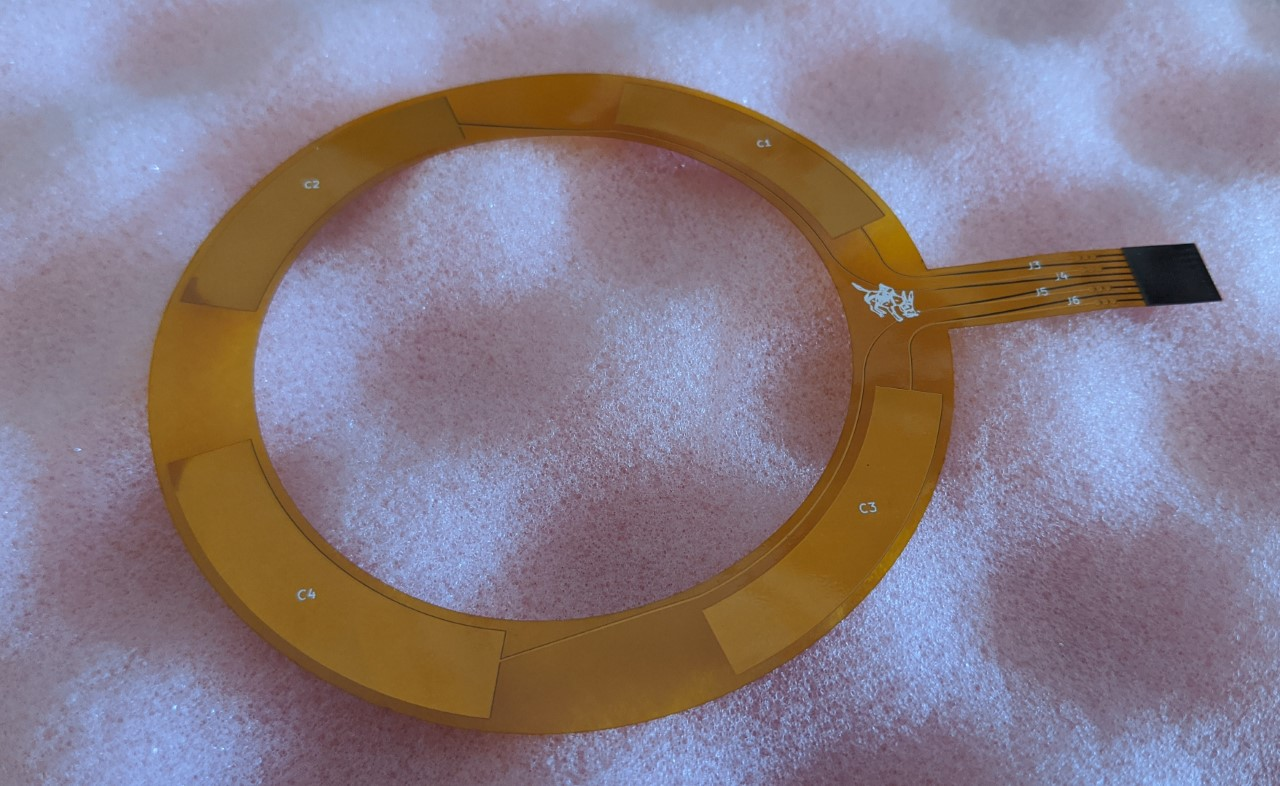
\includegraphics[width=0.7\textwidth]{sensorpic.jpg}
\caption{The dynamic flexible PCB capacitive load cell. 
This sensor is used for the first branch of this research.
It has a thin film layer between the electrodes made of polyimide 
that deforms when pressure is applied. The sensor is housed in a steel case for
protection and additional stiffness and protection from electro-magnetic interference.
}
\label{fig:flexcell}
\end{figure}
